\section{Discussion}

\subsection{Retrospective Characteristics}
One of our research objectives was: \textit{What are the main characteristics in current retrospective practices, in
terms of outcome, processes and impediments?} Throughout this section we will provide a descriptive discussion on the characteristics we have identified throughout our studies. The section is split into three parts: Output, Process Characteristics and Impediments. An overview of all the characteristics can be seen in \autoref{table:retrospective-properties}

\begin{table}[h]
	\begin{center}
		\caption{Retrospective characteristics}
		\label{table:retrospective-properties}
		\begin{tabular}{p{0.9\textwidth}}
			\hline
			\textit{Retrospective Characteristics}\\
			\hline
			\textbf{Output} \\
			Reflection on work processes, technical issues, work environment \\
			Creates improvement opportunities \\
			Improvement implementation \\
			Provides organizational learning \\
			Can improve team enthusiasm \\
			Can decrease team enthusiasm \\ 
			Can improve efficiency  \\
			Facilitates empowerment \\
			\hline 
			\textbf{Process Characteristics}\\
			Little considerations taken \\
			Wish to improve \\
			Varying techniques\\
			Occurs regularly\\
			Collects opinions from participants\\
			Arena for open discussion \\
			Allows for experiments in work environment\\
			Shared learning event\\
			\hline
			\textbf{Impediments}\\
			Team commitment\\
			Enforcing of process improvement actions\\
			\hline
		\end{tabular}
	\end{center}
\end{table}

\subsubsection{Output}

\paragraph{Creates Improvement Opportunities}
Through our studies we have seen that teams are able to improve based on decisions created during the retrospective. From the depth study of Team Zulu we saw that through 77 retrospectives the team had created 343 actions which reflect improvement opportunities. Also all the teams in our breadth study created actions to improve some aspect of their work-life. It is clearly evidence that improvement opportunities are created through the retrospective. This seems to fit well with previous research \cite{Larsen2006, Dingsoyr2004, Drury2012} that the retrospective help identify improvement opportunities. 

\paragraph{Improvement Implementation}
The question if the improvement opportunities are actually implemented can also be seen through our studies. The results of our studies revealed that most of the teams were satisfied with their implementation rate. From team Zulu we learned that only 65 of the 343 actions were not yet implemented. It was also revealed that implementation could be a challenge, as was the case with team Charlie. We identified two methods that seemed to help overcome this challenge. The first was assigning responsible team members to each action. The second was SCRUM master follow-up of the actions. We have seen that retrospective practicing agile development teams are able to implement improvement opportunities confirming Derby and Larsen's \cite{Larsen2006} statement of retrospective helping team adapt. This is contradicting the research of Drury et. al. \cite{Drury2012} which finds that no real changes occur as a result of the retrospective. 

\paragraph{Can Improve Efficiency}
The retrospective practice can, as we have seen in multiple examples, improve the efficiency of teams conducting them. Team Echo's practice changes from SCRUM to KANBAN and then to modified SCRUM and Team Zulu's ``Bug-crunch day'' are just two of the examples we have seen that the teams have been able to improve their efficiency through the retrospective practice. This again confirms the previous literature \cite{Dingsoyr2004, Larsen2006, Kinoshita2008} that retrospectives are able to improve practices and contradicts the finding of Drury et. al. \cite{Drury2012} that retrospectives provide no real changes.

\paragraph{Allows for Experiments in the Work Place}
\label{section:experiments-in-work-place}
As seen in \autoref{section:Derby-Larsen-Structure} a retrospective can be an area that facilitates experimentation in a team. We have observed this, for example as described with team Echo in \autoref{question-11}. Here team Echo tried to move to KANBAN from SCRUM, the experiment was not an immediate success, but allowed them to return to a SCRUM methodology that they could tailor after their experiences from the experiment. This resulted in their work methodology fitting their team better. Our work with team Zulu also led to experimentation, for example their decision to create a dashboard to log their retrospective actions. Another experiment by team Zulu was the inclusion of a ``bug-crunch'' day seen in \autoref{question-11}. This experiment was a success and led to a noticeable decrease in bugs.

\paragraph{Shared Learning Event}
The theory of the retrospective as a shared learning event was described in \autoref{intro:retro-outcome}.  An example of a shared learning event from the same section was performed by team Delta, as they changed their time estimation practices to great success after discussing the process in a retrospective. However none of the teams interviewed made an organized effort to make the result of the retrospective a learning event for personnel outside the team, as recommended by Dingsøyr ~\cite{Dingsoyr2004}.

\paragraph{Enthusiasm}
\label{section:positive-loop-enthusiasm}
Team enthusiasm is both affected by the retrospective practice and inflicted by it. It can be increased through a positive feedback loop or decreased by a negative feedback loop. As a result of the retrospective practice individual empowerment is facilitated and this also increases the enthusiasm. We will describe and discuss each of these statements below through examples from our studies and earlier literature. 
\label{posi-loop}
We have seen that the enthusiasm of the participants of retrospective practice can be both affected by the retrospective. We uncovered a positive loop that helps increase the enthusiasm of the team conducting retrospectives. If changes occurred as a result of the retrospective the participants would become enthusiastic and thus the chance of more changes would occur. Ownership towards the development process was one factor that could help increase the enthusiasm and feed the positive loop. This positive loop confirms what Derby and Larsen \cite{Larsen2006} states that teams are invested in the success of improving their work as the improvements are chosen by the teams themselves and not from upper management. 
\label{negi-loop}
The retrospective practice has also the ability to decrease the enthusiasm of the practicing team. As the opposite of the positive loop a negative are able to decrease the enthusiasm. If no changes occur enthusiasm will decrease and as the enthusiasm decreases the chance of new changes occurring decreases. Some even might see the retrospective as a waste of time as described by team Charlie's SCRUM master which had happened with some of the teams in his department. This confirms our previous literature review \cite{Dolvik2014} that recurring issues kill the joy and Drury et. al. \cite{Drury2012} research that some may see the retrospective as a waste of time. 

\paragraph{Facilitates Empowerment}
Ownership towards the development process was seen as crucial towards getting improvement out of the retrospective by the interviewed teams. Each team member has the possibility to participate in shaping their working process through the retrospective. As seen in team Alfa and Echo even the shy are required to participate in returning feedback and contribute solutions for current work processes. Tessem \cite{Tessem2014} identifies participation in process improvements as an empowering practice. This directly relates to the retrospective practice, which is also a parallel drawn by Tessem and our work supports this. Enthusiasm is increased as members are empowered\cite{Tessem2014} and thus the retrospective increase enthusiasm through empowerment. 

\subsubsection{Process Characteristics }

When we consider our results we see that few of the teams interviewed do a thorough consideration of their practices in relation to the approaches seen in \autoref{table:postmortem-approach}. Most teams did not do a informed decision on several of Dingsøyr's considerations. For example on who to invite or sharing tacit and explicit knowledge. For example team Alpha's interviewee said that it could go long periods of time where a developer was not invited to a retrospective. When it comes to sharing the knowledge generated none of the teams made a concerted effort to share the knowledge further in their organization that came as a results of learning through the retrospective.

Many teams had a great wish to improve. As seen throughout our results the need to build a culture that allows for learning is absolutely essential for a productive environment. This is in accord with  Dingsøyr's work. Especially trust between the team members emerged as critical for reaching the maximum potential of a retrospective session. An example of the possible improvements is the team dynamic improvements experienced by team Delta when one of their team members brought up the problem that he was not getting help from other team members, as described in \autoref{question-21}. Also after our depth analysis with team Zulu their eagerness to improve let them turn the results from our analysis into a basis for multiple actions intended to improve the team's learning capabilities. 


\subsubsection{Impediments}

Some personalities could provide obstacles for the retrospective. We saw three examples of this. The first one was in team Zulu where cultural differences provided miscommunication and difficulty providing an open discussion in the retrospective. The second was in the department to team Charlie where some SCRUM masters had low enthusiasm for the retrospective practice and this could influence the rest of the teams as well. The third example were two senior developers with strong personalities, in team Charlie, that could hinder the other developers from voicing their opinions. These were the only three cases we saw in our studies, but further personalities may be investigated. Derby and Larsen \cite{Larsen2006} talks about personalities that take a lot of time and hinder others from taking part in the retrospective and this is reflected pretty well in the last example.

Even though most of the teams in our study was satisfied with the commitment from their teams, implementation of actions still could provide a challenge. As mentioned by several of the interviewees if the actions were not assigned to a specific person the action would not be implemented. This indicates that the team as a whole don't have the commitment to implementation of retrospective actions. Drury et. al. \cite{Drury2012} described several obstacles that fit with these results. Team members unwilling to commit and relying on SCRUM master, not implementing decisions or relying on others for decisions, and not taking ownership of decisions are all obstacles that could be identified through our research. However as mentioned this was only the case when the group as whole was assigned to a decision, when individuals of the group were assigned the teams were satisfied with the implementation rate. This still indicates however a lack of team commitment even though the consequences are dealt with. 

Enforcing the implementation of process improvement actions was seen as a challenge. The SCRUM master of team Zulu described how enforcing and monitoring process improvement actions was a challenge. Some process changes required the whole team to implement the action and both enforcing the implementation and monitor it could be hard. Conflicting priorities and not taking ownership for decisions are two of Drury's et. al. \cite{Drury2012} obstacles to effective decision making, and these results reflects the two obstacles. 

The last impediment we have seen for conducting retrospective is availability. In team Golf we saw how having a distributed team could make it harder to conduct the retrospective. In team Alfa and Foxtrot we learned how the unavailability of retrospective due to long timespan or participants not being able to participate could inhibit the retrospective. Zedtwitz's \cite{Zedtwitz2002} barrier of memory bias and Drury et. al. \cite{Drury2012} obstacle of unavailable staff is reflected in this. 

\subsection{Organization Learning}
One of our research objectives were: \textit{How is learning achieved through current retrospective practices, in light of organizational learning theory?} Throughout this section we will first discuss the results of our case-studies in terms of the governing values of Argyris and Schön's \cite{Argyris1996} organizational learning Model I and Model II. Secondly we will discuss our results in terms of learning types. 

\paragraph{Model I Summary}
The governing values from Argyris and Schön's Model I seems to not occur or be the system employed by agile development teams performing retrospective systems today. We have only seen two cases where the governing values of Model I have had any implications on the teams. The first one was that of face-saving from one of the team members resulting in an atmosphere suppressing the other member's feelings. This member later left the team. The other implication of Model I governing values is that of single-loop learning which most teams experience and will be discussed further in \autoref{discussion:learning-types}

\begin{table}[h]
	\begin{center}
		\caption{Governing values and consequences encountered in relation to retrospectives.}
		\label{table:model-i-occurences}
		\begin{tabular}{l l}
			\hline
			\textit{Model I} & \textit{Encountered} \\
			\hline
			\textbf{Governing Values} & \\
			Defined goals and try to achieve them. & No \\
			Maximize winning and minimize loosing. & No \\
			Minimize generating or expressing negative feelings & No \\
			Be rational & No \\
			\hline
			\textbf{Behavioral World Consequences} & \\
			Defensive actors & Once observed \\
			Defensive interpersonal and group relationship & No \\
			Defensive norms & No \\
			\hline
			\textbf{Learning Consequences} & \\
			Self-sealing & No \\
			Decreased long-term effectiveness & Not observed \\
			Single-loop learning & Yes \\
			Little testing of theories publicly & No \\
			Much testing of theories privately & No \\
			\hline
		\end{tabular}
	\end{center}
\end{table}

\paragraph{Model II Summary}
The governing values and it's consequences for Argyris and Schön's Model II of organizational learning systems are both apparent and absent from agile teams and retrospectives. Valid information and free and informed choice are both seen in retrospectives. Internal commitment and implementation is also seen, but regarded as a challenge by the teams conducting retrospectives. The behavioral consequences this yield are relationships between actors and the actors themselves are less defensive, learning oriented norms and high freedom of choice and risk taking. The learning consequences from retrospectives are frequent public testing of theories and disconfirmable processes. Double-loop learning is seen in some teams, but not in others. In general the retrospective practice and teams that are conducting them are approaching an Organizational learning II system with some impediments still apparent in the practice.

\begin{table}[h]
	\begin{center}
		\caption{Governing values and consequences from Argyris and Schön's Model II encountered in relation to retrospectives.}
		\label{table:model-ii-occurences}
		\begin{tabular}{p{0.7\textwidth} p{0.3\textwidth}}
			\hline
			\textit{Model II} & \textit{Encountered} \\
			\hline
			\textbf{Governing Values} & \\
			Valid information & Yes \\
			Free and informed choice & Yes \\
			Internal commitment & Challenge for some teams \\
			Monitoring of choice implementation & Challenge \\
			\hline
			\textbf{Behavioral World Consequences} & \\
			Actors minimally defensive & Yes \\
			Minimally defensive relations and group dynamics & Yes \\
			Learning-oriented norms & Yes \\
			High freedom of choice, internal commitment, and risk taking & Yes, but internal commitment is a challenge for some teams \\
			\hline
			\textbf{Learning Consequences} & \\
			Frequent public testing of theories & Yes \\
			Disconfirmable processes & Yes \\
			Double-loop learning & Appearing in some teams, absent from others \\
			\hline
		\end{tabular}
	\end{center}
\end{table}

\subsection{Learning Types}
\label{discussion:learning-types}
Of the three learning loops described in \autoref{intro:organizational-learning} some were more occurring than others in our studies. From team Zulu we learned that 66.4\% of the actions were a single-loop learning result. 27.2\% found the influences of the issues and fixed them resulting in double-loop learning. In total only four of the teams studied had any focus on root-cause and double-loop learning. Only two of the teams had some reflection on how they learned from the retrospective, which is triple-loop learning.

We find these learning results surprising as Model II is supposed to facilitate double-loop learning. As most of the governing values are in use during the retrospective one could assume that double-loop learning would occur more. Especially as most of the teams had a wish to do so. Of all the teams only Alfa seemed to perform double-loop learning on the issues they discussed, however they only discussed the most pressing issues. Team Zulu performed double-loop on about a third of the issues and team Delta found the root-causes on issues they found important. Drury et. al. \cite{Drury2012} found that operational daily tasks are prioritized above tactical and strategic ones and this can seem to be one possible reason for not doing double-loop learning. Teams may simply find solutions to current problems and not investigate if these problems can occur again and if some extra measures taken should be created to avoid them. 

Ideally every issue should result in some double-loop learning. However in a realistic world, where time is a valuable resource, taking the time to investigate every issue to its root-cause and implementing a solution can be difficult. Especially if external pressure to perform is present. This can askew the focus of the retrospective and result in only single-loop learning being the result from it. It would be interesting to see which types of issues is most important and should be given the time to conduct double-loop learning. In team Alfa and Bravo they voted on which issues they found most important and this could be a good indicator on which issues to dig deep into. However we have not been able to get data on this, but it could make an interesting topic for future studies.

We have seen that triple-loop learning was not apparent in any of the teams except Alfa and to some degree Charlie. Team Alfa was in general very satisfied we their practice of retrospective and also indicated that they perform learning so that issues will not recur, thus double-loop learning. We believe that this provides an example of triple-loop learning and reflection on the retrospective helps teams focus the retrospective and improve the learning value from it. Through our feedback-sessions with Team Zulu we have reflected together with the team and provided an arena for triple-loop learning, reflecting on how they conduct their retrospectives. The final feedback-session revealed that the team had decided to keep a better focus on doing double-loop learning and include more positive issues, strengthening our assumption that triple-loop learning helps focus the retrospective. That our interview subjects also responded that it was a good idea and should be done, strengthens this as well.

The three learning types single-, double-, and triple-loop learning can all be a part of the retrospective practice. In our study we have seen that most issues discussed during the retrospective results in single-loop learning, even though they are approaching a Model II learning system. Some teams are able to do double-loop learning on issues they find important, like Alfa, Delta, Echo and Zulu. Triple-loop are not seen much during the retrospective. In team Zulu it helped focus the retrospective, and as team Alfa was doing reflection and managed to do double-loop learning we assume that this triple-loop learning helps facilitate double-loop learning and focus the retrospective.

\subsection{Impediments for Learning}
\label{discussion:learning-impediments}
Through our studies we identified several impediments for learning. 

\begin{table}[h]
	\begin{center}
		\caption{Learning impediments}
		\label{table:learning-impediments}
		\begin{tabular}{p{0.3\textwidth} p{0.7\textwidth}}
			\hline
			\textit{Impediment} & \textit{Description} \\
			\hline
			Lack on focus for double-loop learning & Tries to find a solution to issue, rather than prevent it to occur again. \\
			Difficult to generalize & Create general rules for specific events. \\
			No reflection on learning & The lack of triple-loop learning in teams inhibits the team from improving their learning practices. \\
			Internal commitment & Participants that don't contribute or help implement actions prohibit learning as the team will miss feedback. \\ 
			Low enthusiasm & Learning decreases if the participants are not motivated to do retrospective. Provides negative feedback loop. Low enthusiasm gives no changes which gives lower enthusiasm. Creates low internal commitment. \\
			Little action implementation & Creates lower enthusiasm. \\
			Tacitness of process knowledge & Makes it difficult to get an objective view on current state of working practice. \\
			Bureaucratic overhead & Issues that require a lot of resources to investigate or implement solutions for, could be stopped by management. \\
			External Factors & Issues that relate to some external factors like other teams on same project, support or the like can be a challenge to implement solutions for and thus miss feedback from implementation.\\
			\hline
		\end{tabular}
	\end{center}
\end{table}

\subsection{Current State of the Retrospective Practice}
Throughout this study we observed several characteristics and have seen the organizational learning through the retrospective practice. We will now summarize all we have learned through our own framework, where we divided the retrospective into three parts, before, during and after. The framework is described in \autoref{subsubsec:own-framework}. A visualization of this is provided in \autoref{figure:retro-current-state}

\begin{sidewaysfigure}[!h]
	\centering
	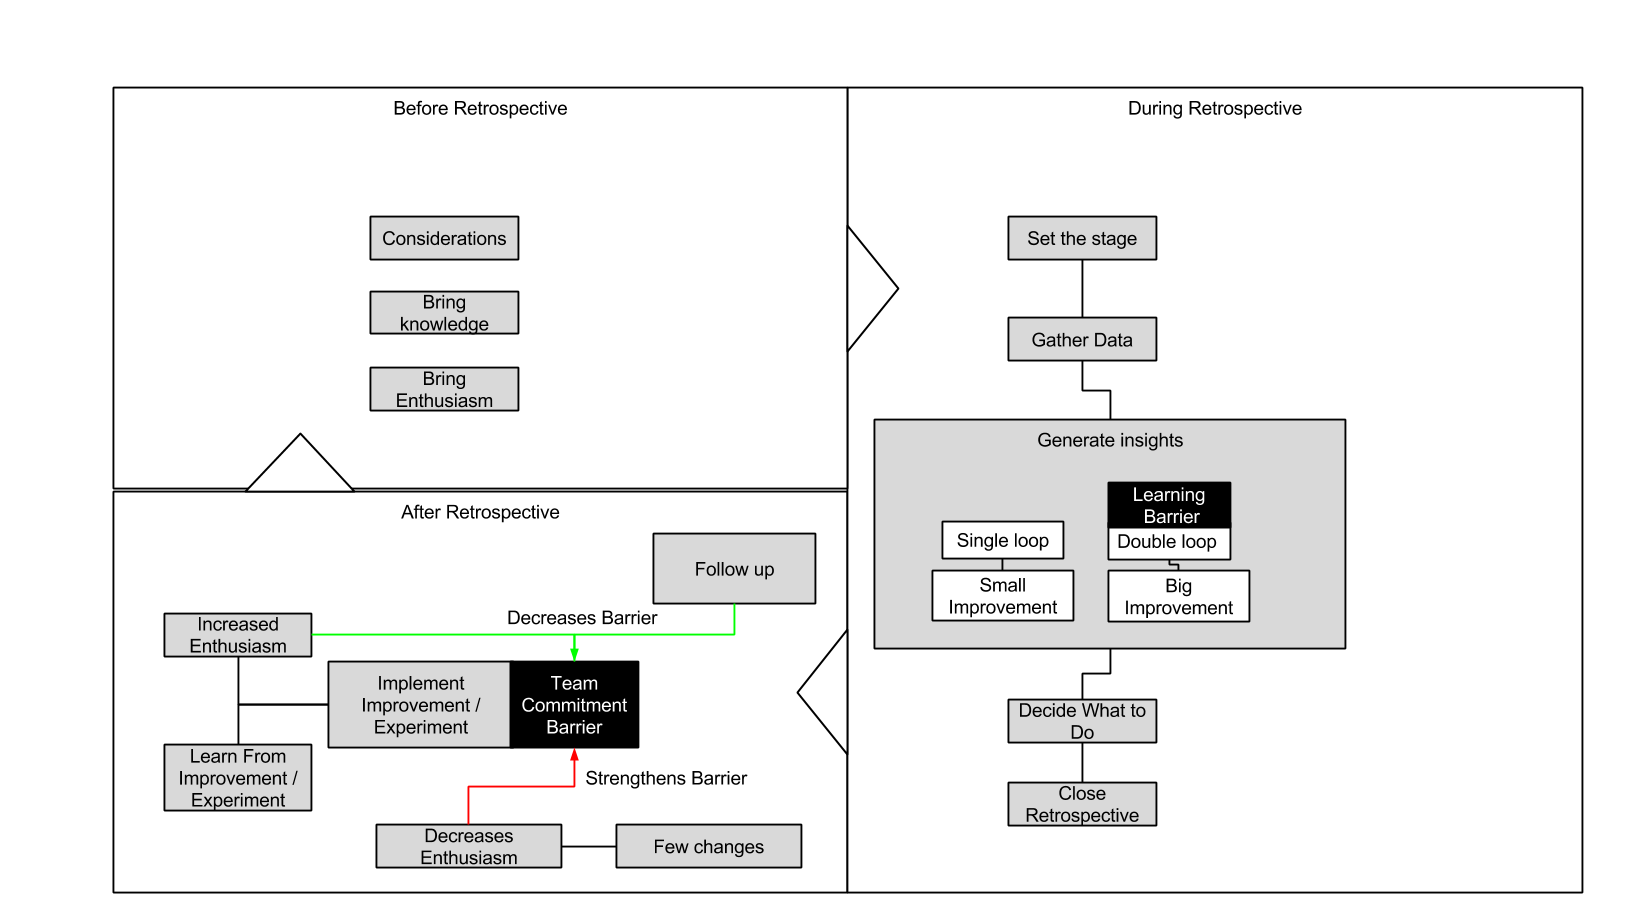
\includegraphics[width=\textwidth, keepaspectratio]{figures/retro-outcome.png}
	\caption{Our perceived state of the retrospective.}
	\label{figure:retro-current-state}
\end{sidewaysfigure}

\subsubsection{Before Retrospective}
The first part of the retrospective practice consists of three elements that we have been able to see through this study: Considerations, bring knowledge and bring enthusiasm. 

Before the retrospective the facilitator or team is required to consider some considerations. Dingsøyr \cite{Dingsoyr2004} proposes several things, however we have seen few of this employed in practice. The considerations we have observed employed by teams today are external facilitator and open or structured discussion. Two of the teams, Echo and Alfa had made the decision to employ an external facilitator. Several of the teams had chosen KJ-Sessions as discussion form, while others just held an open discussion. We have not seen any evidence that any of the teams has made any other informed decision on Dingsøyr's considerations. 

Bringing knowledge and enthusiasm is required by the participants before the retrospective. If no one has any feedback from the last development phase then no learning or improvement opportunities could be identified. Enthusiasm could be brought either as negative or positive as we have seen multiple examples of, in among others teams Zulu, Echo and Charlie. If positive enthusiasm is brought, it will feed into the positive loop, described in \autoref{posi-loop}. If negative enthusiasm is brought it will feed into the negative loop described in \autoref{negi-loop}. 

\subsubsection{During Retrospective}
During the retrospective we have seen that Derby and Larsen's \cite{Larsen2006} structure for conducting retrospectives, described in \autoref{section:Derby-Larsen-Structure}, is mostly followed by all the teams in this study. 

``Set the stage'' and ``Close Retrospective'' is not explicitly mentioned by any of the teams except Charlie and Delta, but it is safe to say that they do start and end the retrospective. The three other steps, ``Gather Data'', ``Generate Insights'' and ``Deciding What to Do'' is done by all of the teams in our study. 

While investigating the learning effects, of the retrospective practice, we found that during the ``Generate Insight'' step a learning barrier was present. The learning barrier consists of several learning impediments, which is described in \autoref{discussion:learning-impediments}, inhibits the team's ability to perform double-loop learning and thus big improvement opportunities are lost. Several of the teams, Zulu, Echo, and Alfa, were able to penetrate this barrier however not without extra effort. For the cases were the teams were not able to penetrate the barrier single-loop learning would be the outcome of the ``Generating insight'' step.

\subsubsection{After Retrospective}
The final part of the retrospective practice is after the retrospective. In this part several new findings revealed a more complex picture than the previously assumed elements of ``Learning'', ``Improvement'' and ``Enthusiasm''.

We identified a barrier to implementation of improvement opportunities that was strengthened and weakened by several other steps. The barrier consisted of the impediments related to team commitment, described in \autoref{team-commi}. If few changes were the result of the retrospective it could decrease the enthusiasm which would feed into the negative loop, described in \autoref{negi-loop}, and strengthen the barrier. If the team was able to overcome the barrier and see clearly improvements they would be able to learn from these improvements and enthusiasm would be increased. When the enthusiasm increases it would feed into the positive loop, described in \autoref{posi-loop} and decrease the barrier. Another measure to decrease the team commitment barrier were follow-up done by the SCRUM master as this would help implementation of improvement opportunities. 

\subsection{Method Proposal: Meta-Retrospective}
\label{section:Method-propsal}
In this section we aim to discuss the potential of improving the current state of the retrospective in a team. We will propose a method based mainly on our depth study work with team Zulu. This method we decided to call a ``Meta-retrospective''. The intention is to provide a framework for evaluating the current state of a retrospective in a project, and potentially improving the retrospective process as a result. The aim of this process is to decrease the learning barriers affecting the team. An overview figure can be seen in \autoref{figure:retro-meta-state}. This section will describe a process on how a ``Meta-retrospective'' potentially could be conducted.

\paragraph{Motivation for Meta-Retrospective}
After observing that no teams practiced team level reflection of own learning and the retrospective process, as seen in \autoref{section:after-the-retrospective}, we developed the meta-retrospective as a method-proposal. The motivation is based in triple-loop learning, described in \autoref{sub:triplloop} where one reflects on ones own learning process and learns from it. Seeing the results from the feedback sessions with team Zulu and the results of their own internal retrospective on retrospectives we observed that they had created a better focus on how they should benefit most from the retrospectives including more focus on double-loop learning, better monitoring of improvement implementation and a more positive attitude during the meetings. All actions and improvements that will approximate towards an organizational learning II system as proposed by Argyris and Schön \cite{Argyris1996}.

\subsection{Guidelines for Conducting Retrospectives}

Through this study we have identified several characteristics that we believe will have positive impact on the conduction of the retrospective process in a modern team. These will be presented in a set of guidelines, followed by a short explanation of each point.

\begin{itemize}
	\setlength\itemsep{1pt}
	\item External facilitating
	\item Implementation of actions 
	\item Address actions to name and visualize
	\item Enthusiasm
	\item Trust
	\item Ownership
	\item Experimentation
	\item Reflection on own learning
	\item Regular retrospectives
	\item Measured varying of technique
	\item Find root causes
	\item Follow up implementations
	\item Reflect on how to conduct own retrospective
	\item Move beyond day-to-day decisions
\end{itemize}

\paragraph{External Facilitating}
As described in \autoref{section:facilitator} we observed multiple instances in which the use of an external facilitator was positive to the team. There are multiple approaches that could be used to arrange an external facilitator, an example would be switching SCRUM masters between teams in the company, another possibility would be using personnel from outside the company.

\paragraph{Implementation of Actions}
The ensuring implementation of actions appears critical for a team to have confidence and trust in the retrospective process. Therefore attempts to conduct a good retrospective should attempt to ensure that actions are completed, and that this success is acknowledged by the team. As seen in our work with team Zulu this is very possible and can lead to a positive effect in the team. Implementation of actions feeds the positive loop described in \autoref{section:positive-loop-enthusiasm}.

\paragraph{Address Actions to Name and Visualize}
One step we observed that had a major impact on the implementation of actions was the follow-up protocol. In \autoref{table:follow-up-techique} we observe that the teams assigning name to an action are satisfied with their implementation of actions. Another positive step is the visualization of the actions.

\paragraph{Follow up Implementations}
A team should ensure that there is some sort of follow up that ensures that actions are implemented. For example this responsibility can fall to SCRUM master as seen in team Echo in \autoref{question-6}.

\paragraph{Trust}
The building of trust seems absolutely central to unlocking the potential of the retrospective session. Thus a team looking to improve should investigate possibilities relating to increasing the sense of trust between team members. One example of the positive impact this can have on a team can be seen in \autoref{question-21}, where team Delta improves team dynamic through a discussion enabled by the high level of trust in the team.

\paragraph{Ownership}
The generation of ownership has a very positive effect on the team's attitude towards retrospective. This is discussed in \autoref{section:positive-loop-enthusiasm}. In order to facilitate this ownership a team should be empowered in their decision making, leading to them shaping their own work processes into something they own.

\paragraph{Experimentation}
A retrospective should be open to allow experimentation in the following development iteration. We have observed this leads to several benefits for the teams in our analysis, this is described in more detail in \autoref{section:experiments-in-work-place}. 

\paragraph{Reflection on Own Learning}
Through our work we discovered that team level reflection on learning processes has little or no presence. The work done with team Zulu indicates that this reflection can provide benefits, and we elaborate our ideas for this characteristic in \autoref{section:Method-propsal}

\paragraph{Regular Retrospective}
Teams without regular retrospectives can be negatively affected in several ways, as described in \autoref{section:Retrospective-timespan}. Making sure there is not too long between retrospectives decreases the effect of memory bias as described in \autoref{section:valid-information}.

\paragraph{Measured Varying of Technique}
We got a wide range of answers when we investigated the use of techniques in a retrospective, as seen in \autoref{section:retrospective-practices-used}. Thus it seems advisable for a team to experiment with using different techniques in order to discover what works for them. One should be mindful of too much variation, as too much variation could steer focus over to the technique instead of the retrospective session

\paragraph{Reflect on How to Conduct Own Retrospective} % (fold)
A team can improve by reflecting how they can benefit from established theory, for example considering how they compare to Dingsøyr's approach elaborated on in \autoref{section:Dingsoyr-Approach-Introduction}.

\paragraph{Find Root Causes}
As described in \autoref{discussion:learning-impediments} some teams can benefit from increasing their focus on double-loop learning. This can lead to more effective decision making as underlying issues are targeted instead of superficial ones. Some techniques observed to find root causes are described in \autoref{question-13}.

\paragraph{Move Beyond Day-to-Day Decisions}
Our work has seen that a retrospective have a potential to move beyond operational decisions, this is for example shown in \autoref{section:decision-making-zulu}. A team mindful of this potential is better suited to improve from their retrospective.
 
\section{Limitations}
There are several limitations to this study. First and foremost is that the teams participating in the study is only recruited from Scandinavia, which could mean that the results of this study might not reflect for teams other places in the world. 

Also only teams that were willing to participate could be studied. This could be a selection bias that potentially might impact the results.

Another limitation of this study could be the small sample size as we only have had one depth study and only seven interviews in our breadth study. This could mean that the results of this study do not necessarily reflect the general mass of practitioners. 

The final limitation is the researchers own inexperience with this kind of research. This is the first time both researchers have conducted such a study, which could mean that some bias might have occurred.